\documentclass[UTTF8, fontset=ubuntu]{ctexart}
\usepackage{parskip}
\usepackage{graphicx}
\usepackage{float}
\begin{document}
如图.\\
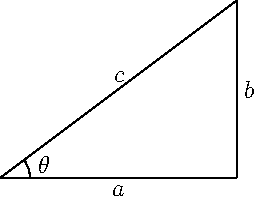
\includegraphics{triangel.pdf}

基本公式列表:\\
\begin{displaymath}
\begin{array}{l l l}
    \sin(\theta)=\frac{b}{c} & \cos(\theta)=\frac{a}{c} & \tan(\theta)=\frac{b}{a}\\
    \csc(\theta)=\frac{1}{\sin(\theta)}=\frac{c}{b} & \sec(\theta)=\frac{1}{\cos(\theta)}=\frac{c}{a} & \cot(\theta)=\frac{1}{\tan(\theta)}=\frac{a}{b}
\end{array}
\end{displaymath}
常见三角函数值:
\begin{displaymath}
\begin{array}{c|c c c c c}
\hline
    & 0 & \frac{\pi}{6} & \frac{\pi}{4} & \frac{\pi}{3} & \frac{\pi}{2}\\
\hline
    \sin & 0 & \frac{1}{2} & \frac{\sqrt{2}}{2} & \frac{\sqrt{3}}{2} & 1\\
    \cos & 1 & \frac{\sqrt{3}}{2} & \frac{\sqrt{2}}{2} & \frac{1}{2} & 0\\
    \tan & 0 & \frac{\sqrt{3}}{3} & 1 & \sqrt{3} & \star\\
\hline
\end{array}
\end{displaymath}

求三角函数值步骤:\\
1.找出角所在象限;\\
2.当角在x/y轴上, 参考三角函数图像;\\
3.如果角不在x/y轴上, 找出该角与x轴形成的最小角度, 即\textbf{参考角};\\
4.当参考角为特殊角时,参考常见三角函数值表;\\
5.利用ASTC(all/sin/tan/cos)决定是否需要添加负号.

三角函数图像:\\
\begin{figure}[H]
\centering
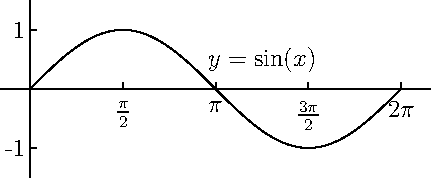
\includegraphics{sin.pdf}
\end{figure}
\begin{figure}
\centering
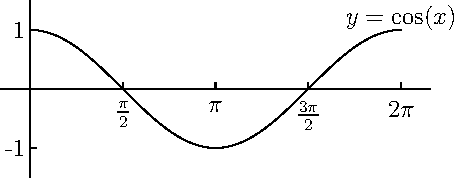
\includegraphics{cos.pdf}
\end{figure}
\begin{figure}
\centering
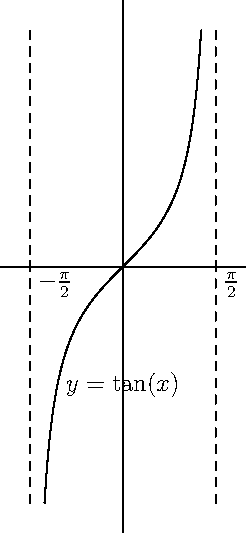
\includegraphics{tan.pdf}\qquad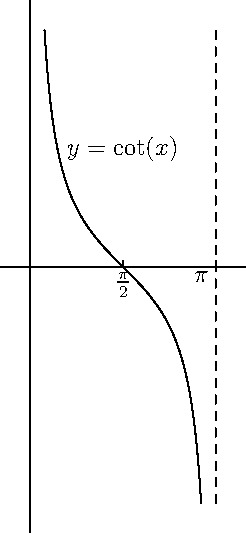
\includegraphics{cot.pdf}
\end{figure}
\begin{figure}
\centering
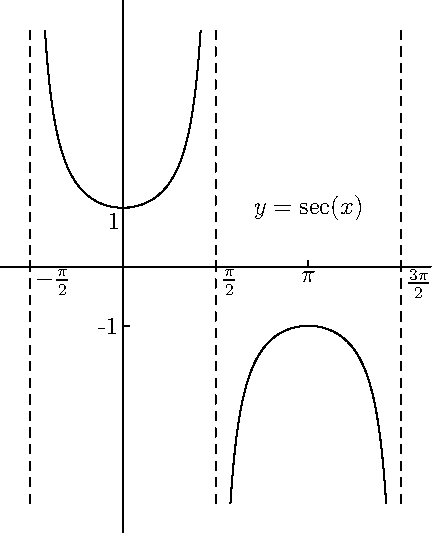
\includegraphics{sec.pdf}
\end{figure}
\begin{figure}
\centering
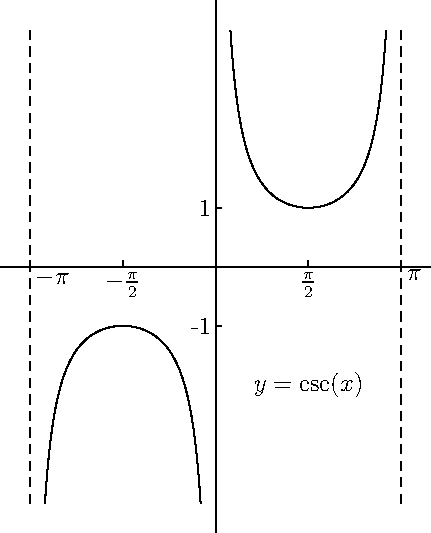
\includegraphics{csc.pdf}
\end{figure}

毕达哥拉斯定理:\\
\begin{center}
\framebox{$\cos^2(x)+\sin^2(x)=1$}
\end{center}
\end{document}
